
\section{Introduction}
The algorithmic trading of stock shares can be triggered by very complex patterns that stock market 
brokers specify based on patterns on event stream of stock market. Such algorithmic trading mostly are specified based on 
history of event stream and by utilizing moving averages of stock prices and trading volumes. The real-time extraction of 
such patterns to trigger buy or sell trading decisions is the task of high-scalable event stream processing systems. 

This year's DEBS Grand Challenge \cite{debs2022challenge} describes a system implementation based on two specific queries 
stock market event streams. The first query computes is defined to compute the Exponential Moving Average (EMA) with two different smoothing factors 
of 38 and 100. Exponential Moving Average is one of the moving averages and is defined as follows:

\begin{align*}
    EMA_t = \begin{cases} 
        Y_0 &  t = 0 \\ 
        \alpha Y_t + (1-\alpha) EMA_{t-1}& t>0 \\ 
        \end{cases}
\end{align*}

The coefficient $\alpha$ represents the degree of weighting decrease, a constant smoothing factor between 0 and 1.
For this challenge $\alpha = \frac{2}{1+j}$ where $j$ is a smoothing factor with $j \in \{38, 100 \}$
$EMA_{38}$ refers to exponential moving average with smoothing factor of 38 and  $EMA_{100}$ has a smoothing factor of 100. 


\begin{figure}[!ht]
    \begin{center}
        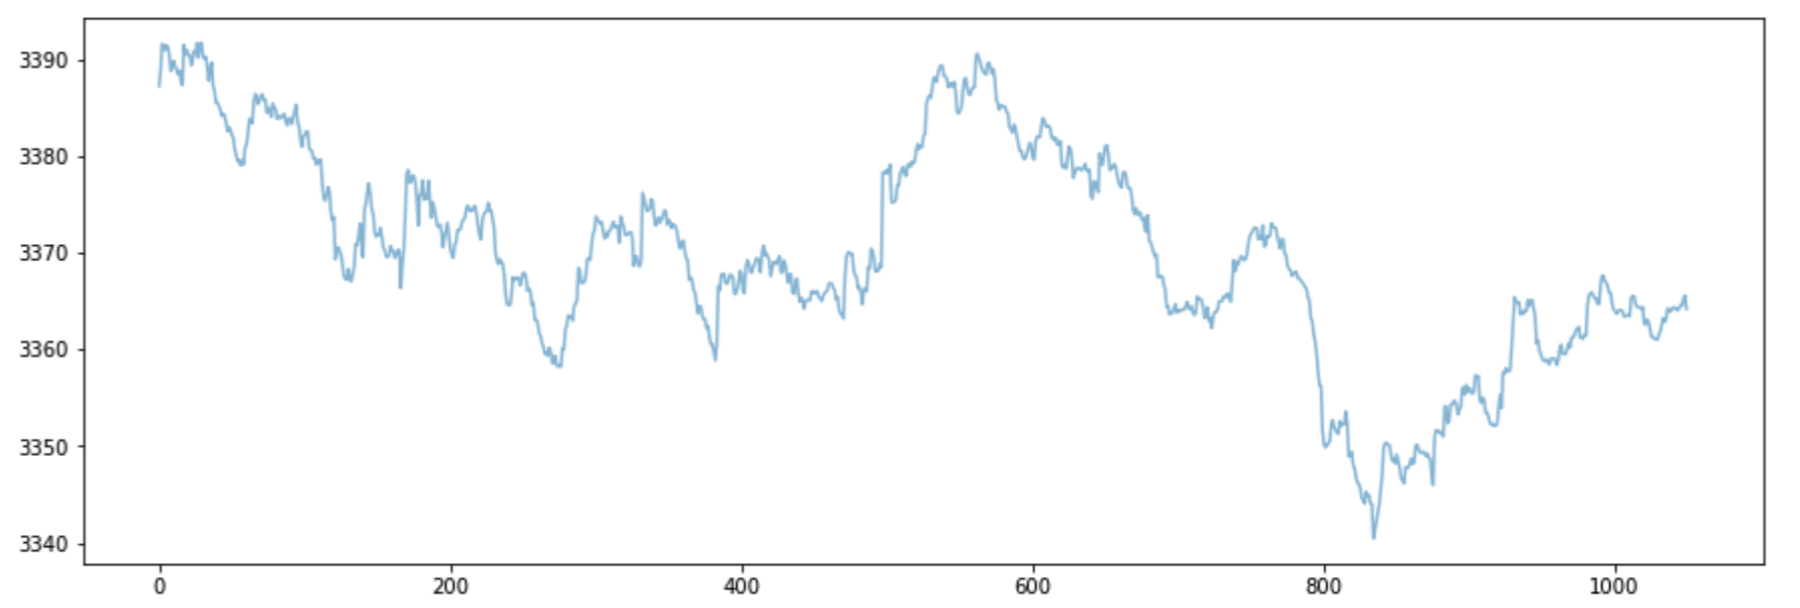
\includegraphics[width=0.42\textwidth]{./images/stock_example.png}
        \caption{An Example of Stock Price Fluctuations Over Time}
        \label{fig:stock}
    \end{center}
\end{figure}



\begin{figure*}[!ht]
    \begin{center}
        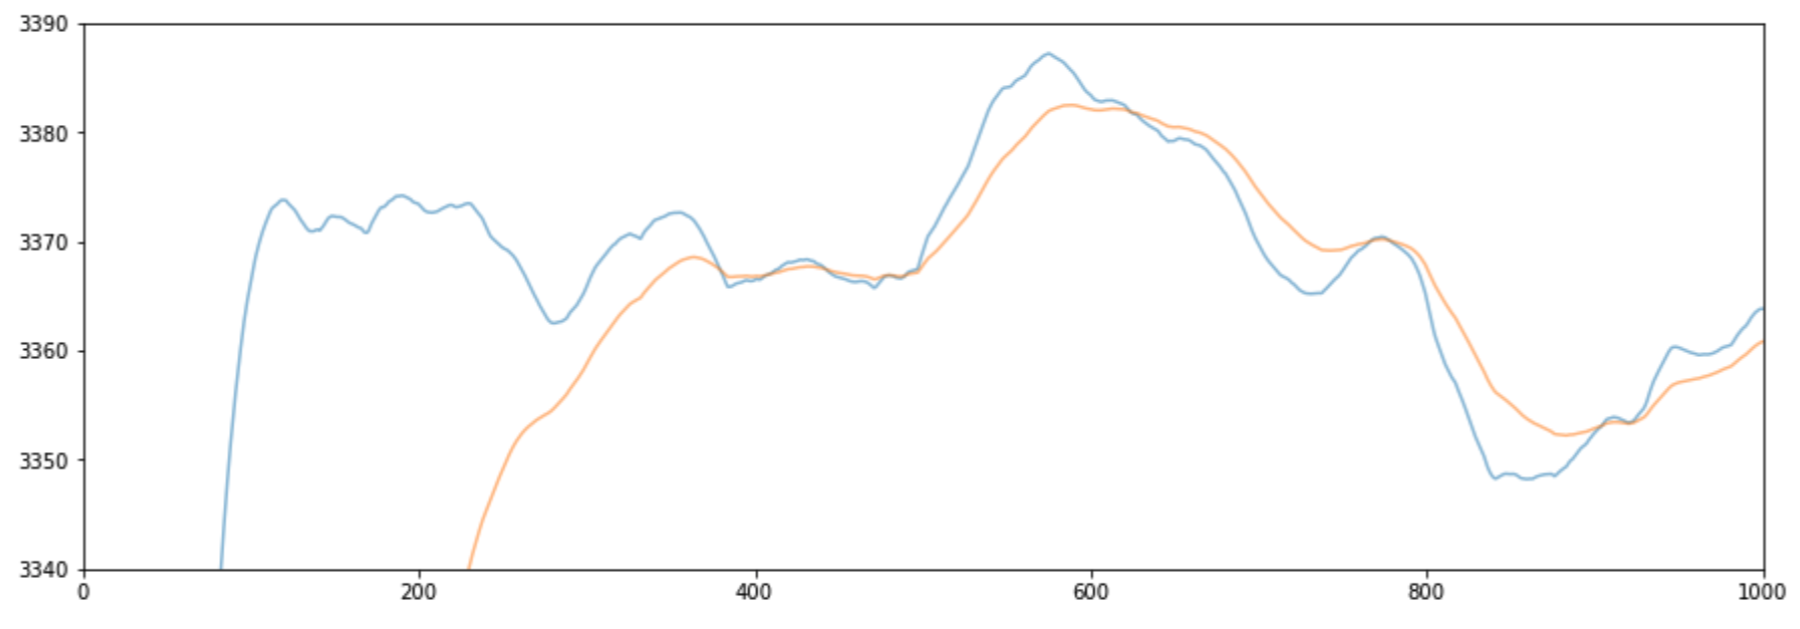
\includegraphics[width=0.90\textwidth]{./images/query2_example.png}
        \caption{Example of Query 2 - Buy and Sell advice based on Breakout Patterns of EMA 38 and 100 }
        \label{fig:EMAs}
    \end{center}
\end{figure*}




Figure \ref{fig:stock} illustrates an example of stock market price changes over time. The graph shows 1000 events with 
different prices. Figure \ref{fig:EMA200} depicts the values of exponential moving average with 
smoothing factors of 38 and 100. We can observe in Figure \ref{fig:EMA200} how the value grows exponentially 
and how the two $EMA_{38}$ and $EMA_{100}$ are different from each other. 


% Describe briefly what the challenge is 

% describe the query 1 

% describe the query 2 


% High-Performance computing problems 
% Scalability issues




\begin{figure}[!ht]
    \begin{center}
        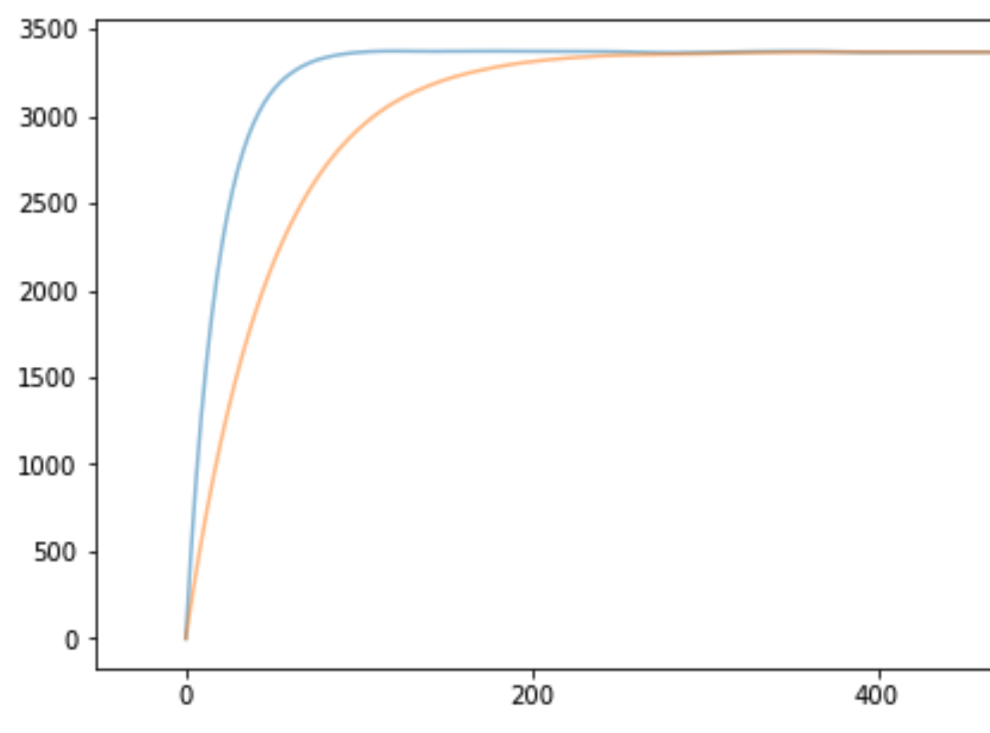
\includegraphics[width=0.42\textwidth]{./images/query2_example_200.png}
        \caption{Exponential Moving Average of 38 and 100 for the first 400 events.}
        \label{fig:EMA200}
    \end{center}
\end{figure}







Spark Streaming \cite{zaharia2010spark}, Apache Flink streaming \cite{alexandrov2014stratosphere}

Esper event stream processing system \cite{Bernhardt2007}


Different data models and serialization have a huge impact on data processing performance \cite{DBLP:conf/cloud/SikdarTJ17}. 

